\section{Weather Dataset}
\begin{comment}
    1) I don't think there should be references to a dashboard in the technical report
    2) What are the variables? If we don't use them, we should not mention them.
    3) The sentence about the API returning parallel hourly arrays is a bit confusing. 
    Parallel is not a very clear term; keeping the historical analysis stable -> what does that mean? Does the use of reanalysis models
    imply that the data has better quality than real-time data / prevision? We should clarify this.
    4) We should better explain the attributes we use, and why we use them. I would have written it as:
    "The dataset includes several attributes. We focused on the following fields, as they are the one that most directly affect ridership". 
    5) Weather timestamps are not downloaded! We request them from the API. 
    The whole paragraph could be written cleaner and moved to the data quality section.
    6) I like the introduction to the analysis and insights section and also figure 8!
    7) Can we report some statistics about the correlation between weather and ridership? 
    E.g., correlation coefficient? This would make the analysis more quantitative and less descriptive.
    8) The data quality section can easily be shortened up, going straight to the point (no missing values, but a big bias)
    It also lack any observation to the found issues. E.g., when computing statisctics for a certian weather condition,
    we might also consider rides that happened in a different weather condition, but were reported as the same due to the bias.

\end{comment}
To enrich the dashboard with meteorological analysis, we incorporate hourly NYC weather data retrieved from the \href{https://open-meteo.com/}{\underline{Open-Meteo archive API}}.

\subsection{Dataset Structure}
Weather data are queried via the Open-Meteo JSON API by specifying coordinates, a date range, and variables.
The API returns parallel hourly arrays derived from reanalysis models that update with a few days' delay, keeping the historical analysis stable in our case.

\subsubsection{Original Structure}
The dataset includes several attributes, but we consider only the following main fields:
\begin{itemize}
    \item \textbf{Timestamp}: Hourly observation time.
    \item \textbf{Temperature}: Air temperature in \si{\degreeCelsius}.
    \item \textbf{Precipitation}: Hourly precipitation in millimetres.
    \item \textbf{Weather Code}: WMO weather condition code.
    \item \textbf{Wind Speed}: Wind speed in km/h.
\end{itemize}

Weather timestamps are downloaded in UTC and converted to local time (\texttt{America/New\_York}) so they match the Citi Bike trip data.
This is done because requesting local time directly applies a single time offset to the whole period, which creates a one-hour error whenever daylight saving time changes.
To prevent missing data after adjusting for local time, we add a one-day buffer to both ends of our search window and trim it back to the exact target dates after conversion.

\subsection{Analysis and Insights}
Weather conditions serve as a key driver of daily bike usage.
Rather than examining weather in isolation, the following section focuses directly on its relationship with overall ridership patterns.

\paragraph{Ridership vs. Weather}
Figure~\ref{fig:rides_vs_weather} illustrates daily ridership alongside mean temperature and total precipitation.
The data shows a clear inverse relationship between precipitation and usage: the month's peak precipitation directly coincides with its lowest ridership volume.
Meanwhile for the temperature, it's possible to see also a positive correlation with ridership, where the rides follows the temperature increase.
This confirms that weather tracking provides valuable context for interpreting demand fluctuations and supporting operational planning.

\begin{figure}[H]
    \centering
    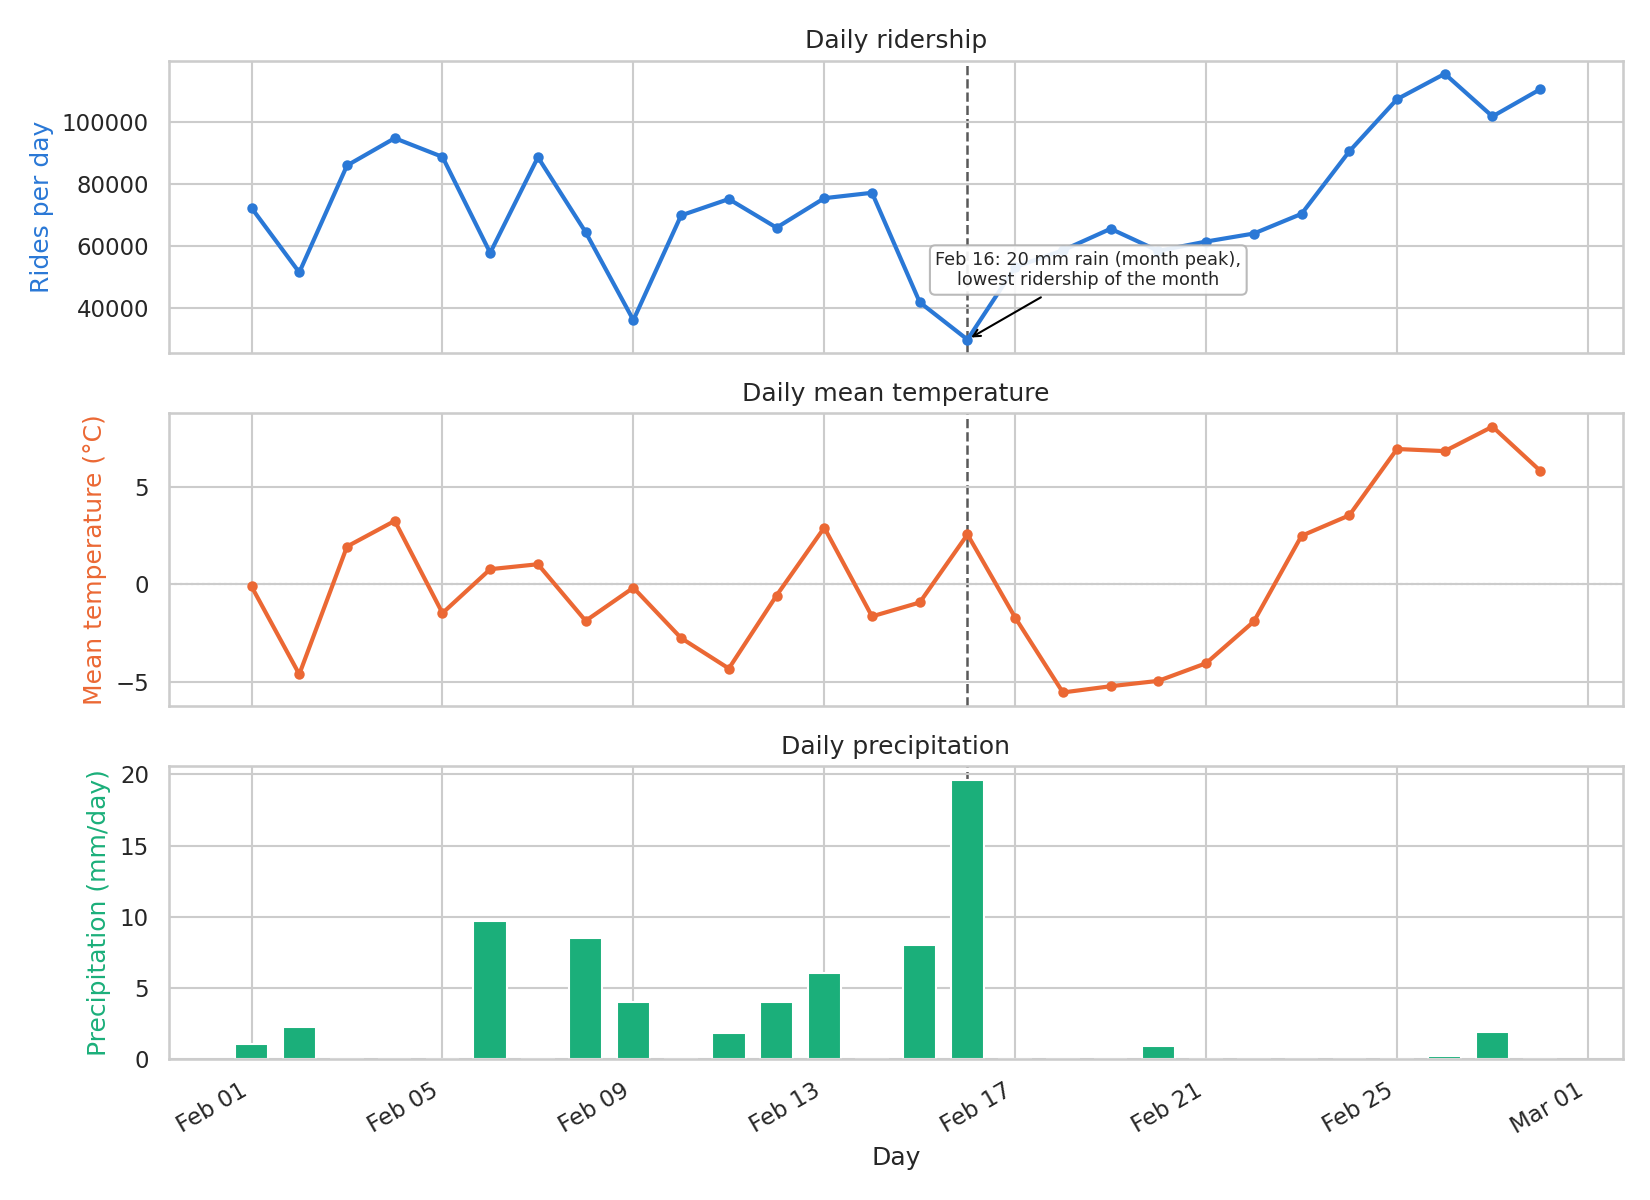
\includegraphics[width=\textwidth]{../media/technical/rides_vs_weather.png}
    \caption{Daily ridership, mean temperature, and total precipitation over the reference month, plotted on aligned date axes with individual scales. The dashed guide highlights 16 February, the month's wettest day and also its least ridden.}
    \label{fig:rides_vs_weather}
\end{figure}

\subsection{Data Quality}
The archive is complete, with an hourly series covering the entire reference year and no missing values in any variable.
The issues we found therefore concern how the values are localised and what they represent, rather than gaps in the data.

\paragraph{Spatial Coverage}
Weather data is retrieved for a single point centered on Central Park and applied across the entire system.
While this dataset misses microclimate variations across a more granular spatial scale, applying higher spatial granularity would introduce more modeling challenges than necessary for a city-scale analysis.
